% this file is called up by thesis.tex
% content in this file will be fed into the main document

%: ----------------------- name of chapter  -------------------------
\chapter{Results} % top level followed by section, subsection
\label{resultsChapter}

This chapter introduces results that were measured from all five programmes, both cycle- and application-level experiments. All reported results are based on ten runs for all buffer sizes. There are multiple figures in the chapter, some of them cannot be rendered on the pages where they are referenced due to their large sizes.

%: ----------------------- paths to graphics ------------------------

% change according to folder and file names
\ifpdf
    \graphicspath{{X/figures/PNG/}{X/figures/PDF/}{X/figures/}}
\else
    \graphicspath{{X/figures/EPS/}{X/figures/}}
\fi

%: ----------------------- contents from here ------------------------

\section{Cycle-Level Experiments}

\label{sec:cycle_results}

\subsection{Experiment 0}

As identified in section \ref{design_env}, it was learnt through running experiments that a number of page faults cannot be avoided for even the shortest experiments. Gathering results that are not affected by the processes that take place in the OS proved to be impossible in the given environment. The act of reading the interrupts count generates page faults. The base Experiment 0 showed that on average accessing data from a CPU register takes 349 clock-cycles.

\subsection{Experiment 1}

Refer to figures \ref{Cycle_experiment_clean_nuim} and \ref{Cycle_experiment_dirty_nuim} for the graphs where unfiltered and filtered (respectively) data measured by running Experiment 1 on the Xeon 5130 is plotted. Filtered data indicates results that are not affected by overhead of the OS; unfiltered data reports measurements as they are seen in the environment, including overhead. On these graphs the x-axes represent the numbers of bytes transferred using the array \textit{testAr}. Data is written/read in a form of \textit{long} words, which are 8 bytes each, on both systems used in the project. The value is defined by the argument \textit{n} that is passed to the experiment function. The y-axes plot how much time (measured in clock-cycles) it takes to write \textit{n} bytes into memory and subsequently read them from memory. Detailed filtered results of first three runs of all iterations of the experiment with an indication of the numbers of interrupts and minor page faults that were recorded while running the experiment in this setting may be found in appendix \ref{app:cycle-level-results-clean-nuim}.

\begin{figure}[!htb]
\centering
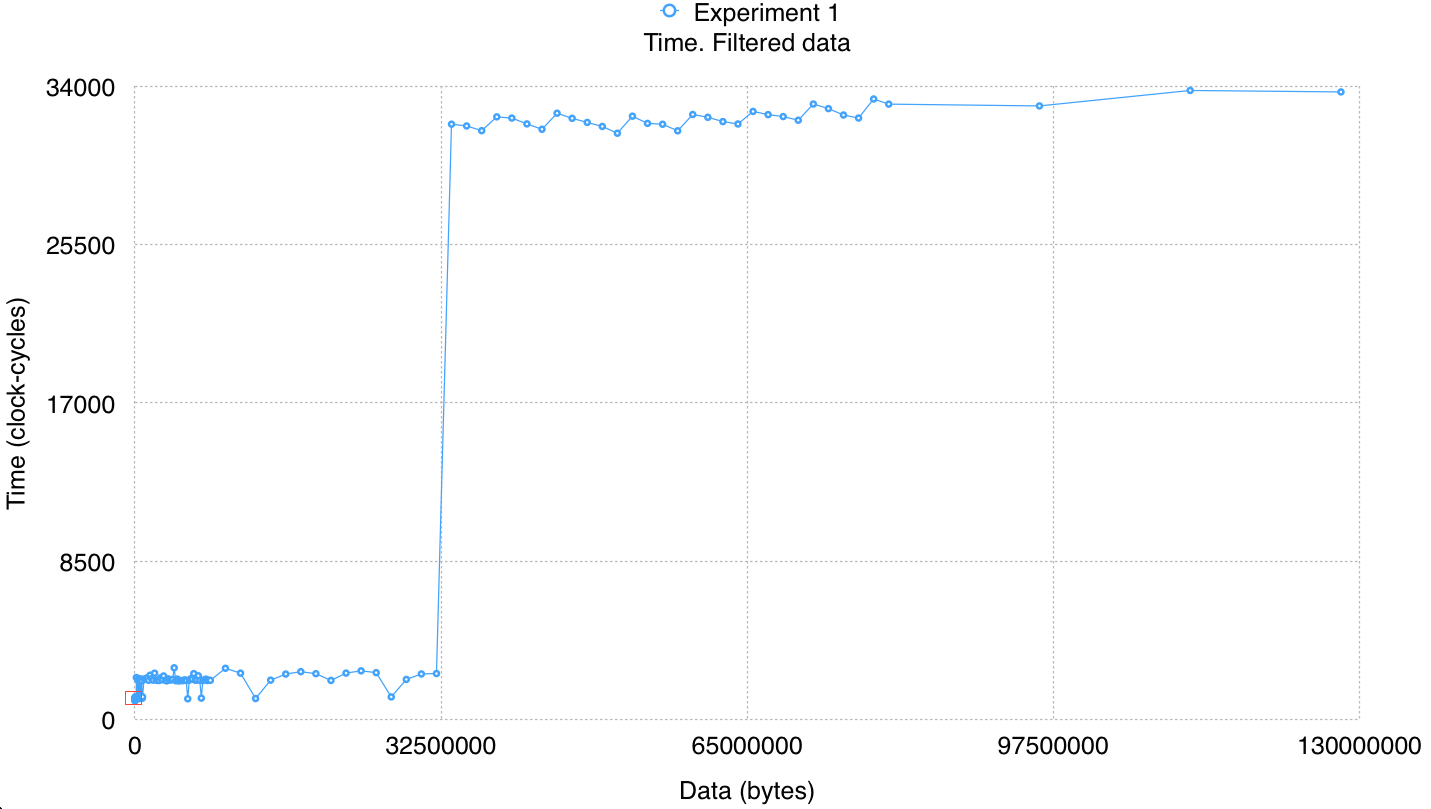
\includegraphics[width=145mm]{6/Cycle_experiment_clean_nuim.png}
\caption{Xeon 5130: data copying times (filtered data, Experiment 1)}
\label{Cycle_experiment_clean_nuim}
\end{figure}

\begin{figure}[!htb]
\centering
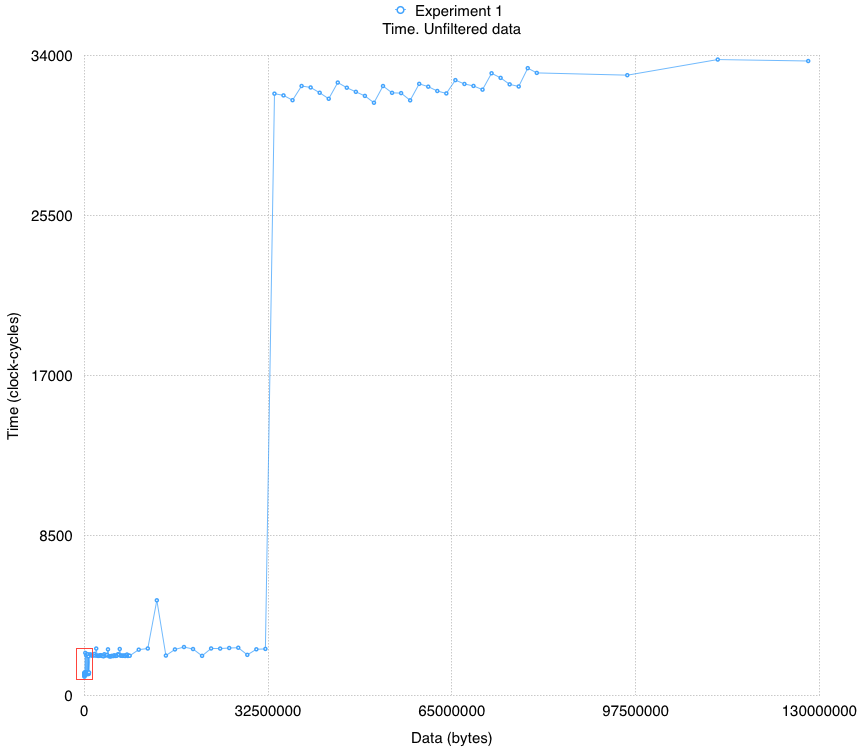
\includegraphics[width=145mm]{6/Cycle_experiment_dirty_nuim.png}
\caption{Xeon 5130: data copying times (unfiltered data, Experiment 1)}
\label{Cycle_experiment_dirty_nuim}
\end{figure}

Figures \ref{Cycle_experiment_clean_nuim_small} and \ref{Cycle_experiment_dirty_nuim_small} are similar to graphs \ref{Cycle_experiment_clean_nuim} and \ref{Cycle_experiment_dirty_nuim}. They also plot filtered and unfiltered data (respectively) measured from running Experiment 1 on the Xeon 5130, but they focus on the results of running the experiment with $8 <= n <= 400064$. The relative parts of the graphs, which are ``zoomed in" are outlined by red rectangles on the figure \ref{Cycle_experiment_clean_nuim} and \ref{Cycle_experiment_dirty_nuim}.

\begin{figure}[!htb]
\centering
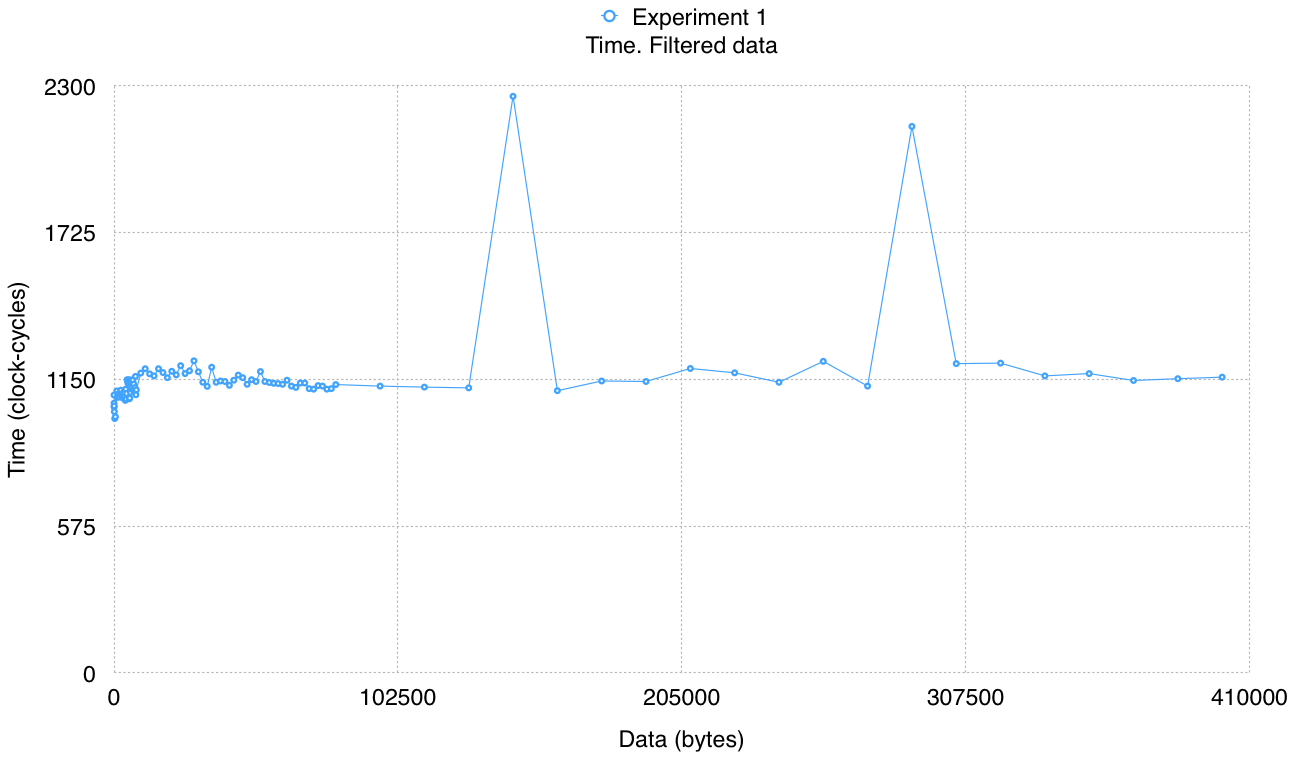
\includegraphics[width=145mm]{6/Cycle_experiment_clean_nuim_small.png}
\caption{Xeon 5130: data copying times, where $8 <= n <= 400064$ (filtered data, Experiment 1)}
\label{Cycle_experiment_clean_nuim_small}
\end{figure}

\begin{figure}[!htb]
\centering
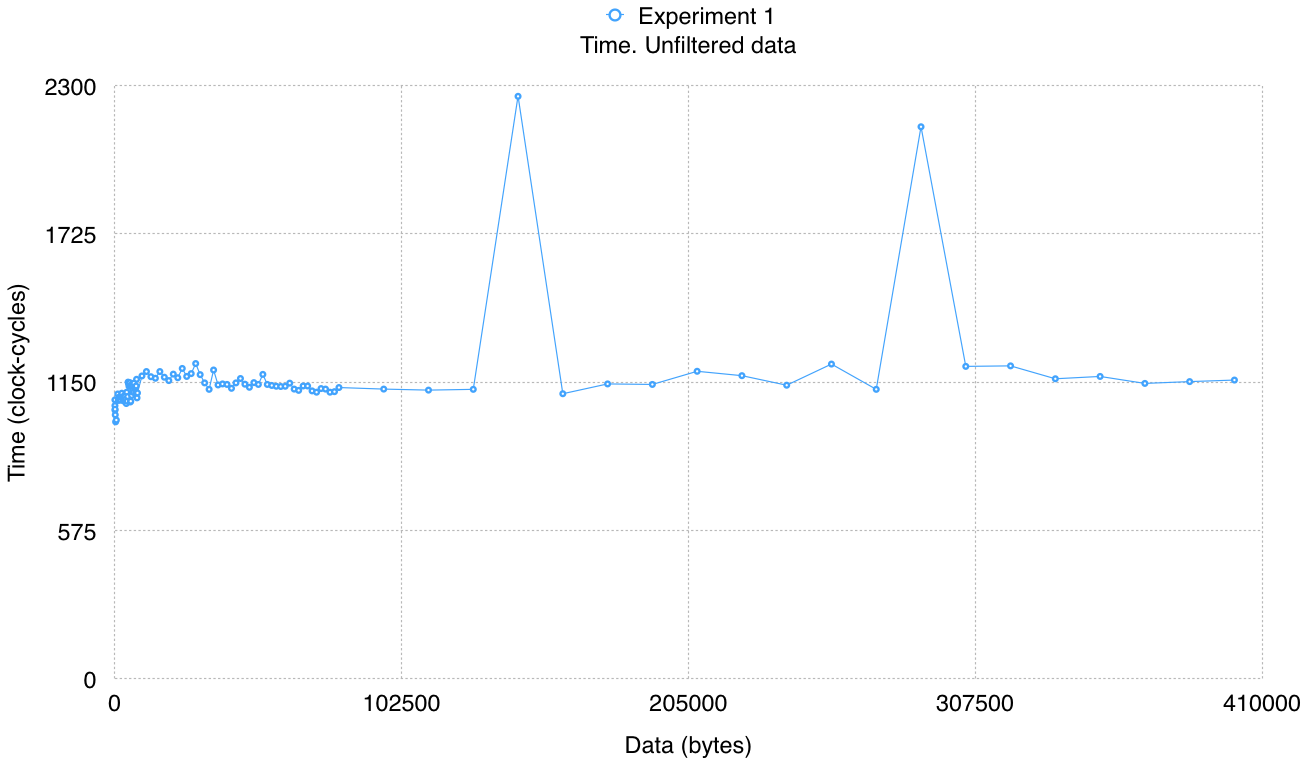
\includegraphics[width=145mm]{6/Cycle_experiment_dirty_nuim_small.png}
\caption{Xeon 5130: data copying times, where $8<= n <= 400064$ (unfiltered data, Experiment 1)}
\label{Cycle_experiment_dirty_nuim_small}
\end{figure}

Refer to figures \ref{Cycle_experiment_clean_ichec} and \ref{Cycle_experiment_dirty_ichec} for the graphs where unfiltered and filtered (respectively) data measured by running Experiment 1 on the Xeon E5-2695 v2 is plotted. As in the case of graphs showing results of running this experiment on a different machine, in these graphs the x-axes represent numbers of bytes written into the array \textit{testAr}. The value is defined by the argument \textit{n} that is passed to the experiment function. The y-axes plot how much time (measured in clock-cycles) it takes to write \textit{n} bytes into memory and subsequently read them from memory. Again, detailed filtered results of first three runs of all iterations of the experiment with an indication of the numbers of interrupts and minor page faults that were recorded while running the experiment in this setting may be found in appendix \ref{app:cycle-level-results-clean-ichec}.

\begin{figure}[!htb]
\centering
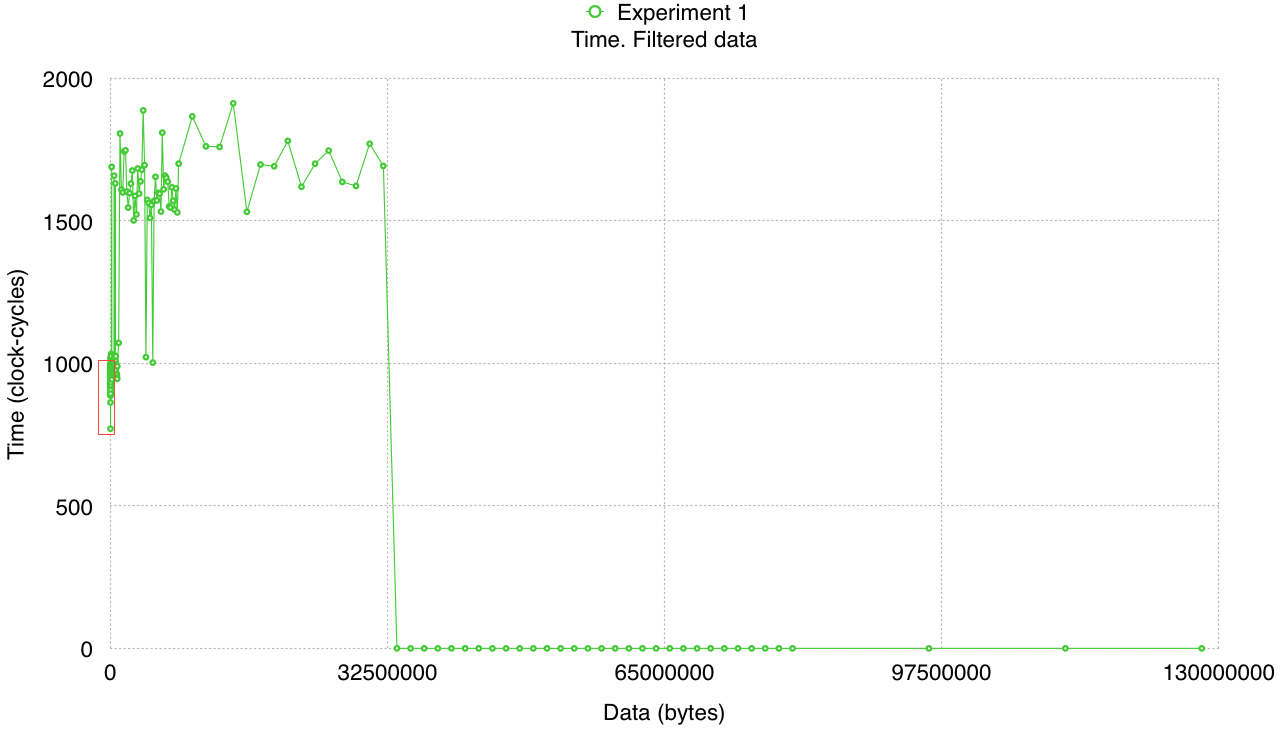
\includegraphics[width=145mm]{6/Cycle_experiment_clean_ichec.png}
\caption{Xeon E5-2695 v2: data copying times (filtered data, Experiment 1)}
\label{Cycle_experiment_clean_ichec}
\end{figure}

Data that was measured on the Xeon E5-2695 v2 was especially ``noisy". It may be caused by the fact that, compared to the Xeon 5130, it is a much more complicated machine where many more processes take place. For $n >= 33600064$, the amount of interrupts and minor page faults generated in the system was so large (at least 4 minor page faults in each run) that all runs of the experiment were seen as ``overly-noisy" data and could not filtered, i.e. all of them are marked as having $t = 0$, where $t$ is execution time.

\begin{figure}[!htb]
\centering
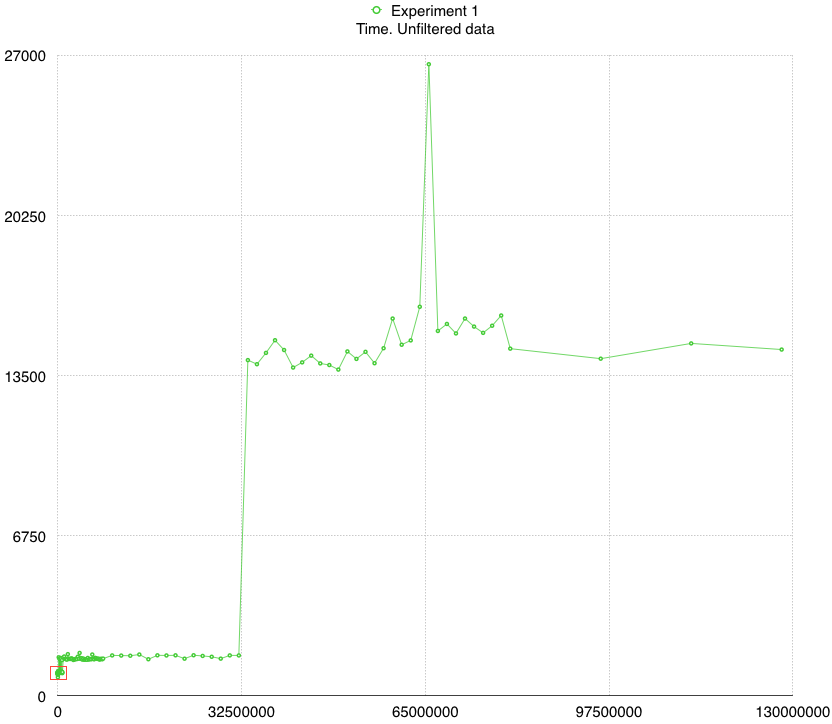
\includegraphics[width=145mm]{6/Cycle_experiment_dirty_ichec.png}
\caption{Xeon E5-2695 v2: data copying times (unfiltered data, Experiment 1)}
\label{Cycle_experiment_dirty_ichec}
\end{figure}

Figures \ref{Cycle_experiment_clean_ichec_small} and \ref{Cycle_experiment_dirty_ichec_small} are similar to graphs \ref{Cycle_experiment_clean_ichec} and \ref{Cycle_experiment_dirty_ichec}. They plot filtered and unfiltered data (respectively) measured from running Experiment 1 on the Xeon E5-2695 v2, but they focus on the results of running the experiment with $8 <= n <= 400064$. The relative parts of the graphs, which are ``zoomed in" are outlined by red rectangles on the figure \ref{Cycle_experiment_clean_ichec} and \ref{Cycle_experiment_dirty_ichec}.

\begin{figure}[!htb]
\centering
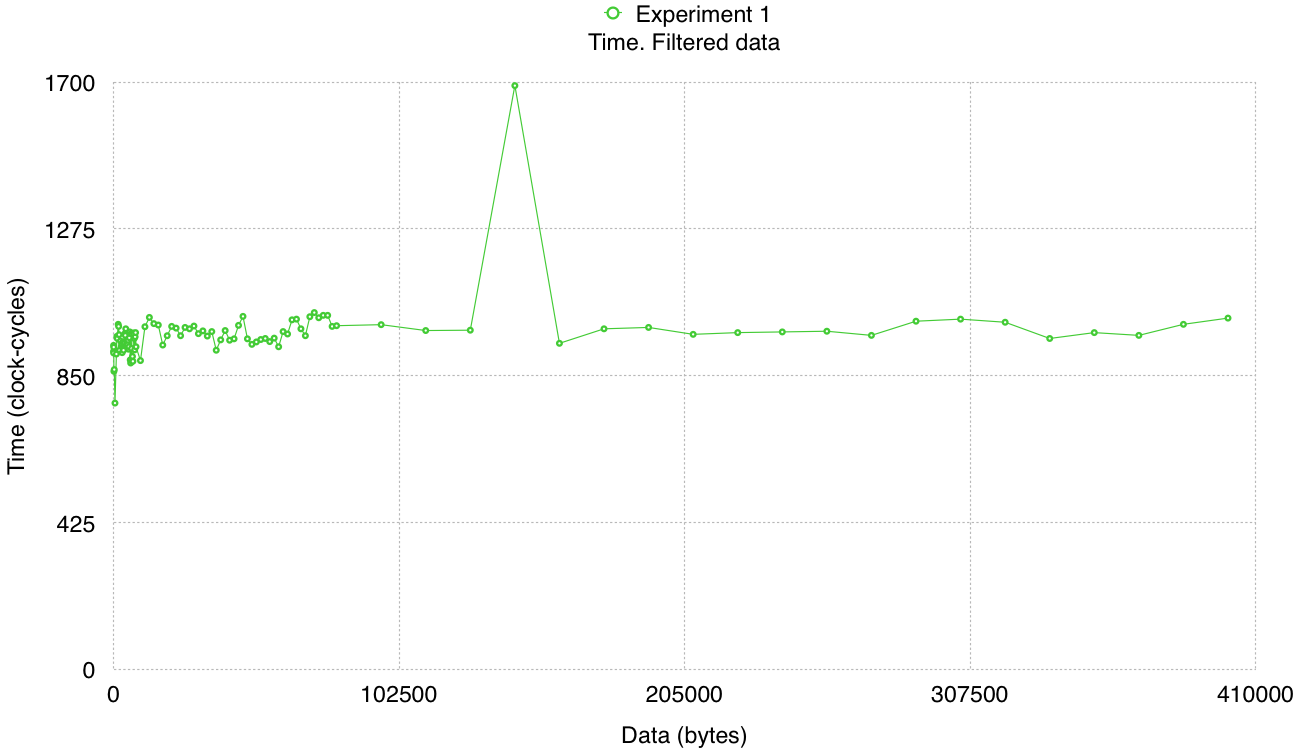
\includegraphics[width=145mm]{6/Cycle_experiment_clean_ichec_small.png}
\caption{Xeon E5-2695 v2: data copying times, where $8 <= n <= 400064$ (filtered data, Experiment 1)}
\label{Cycle_experiment_clean_ichec_small}
\end{figure}

\begin{figure}[!htb]
\centering
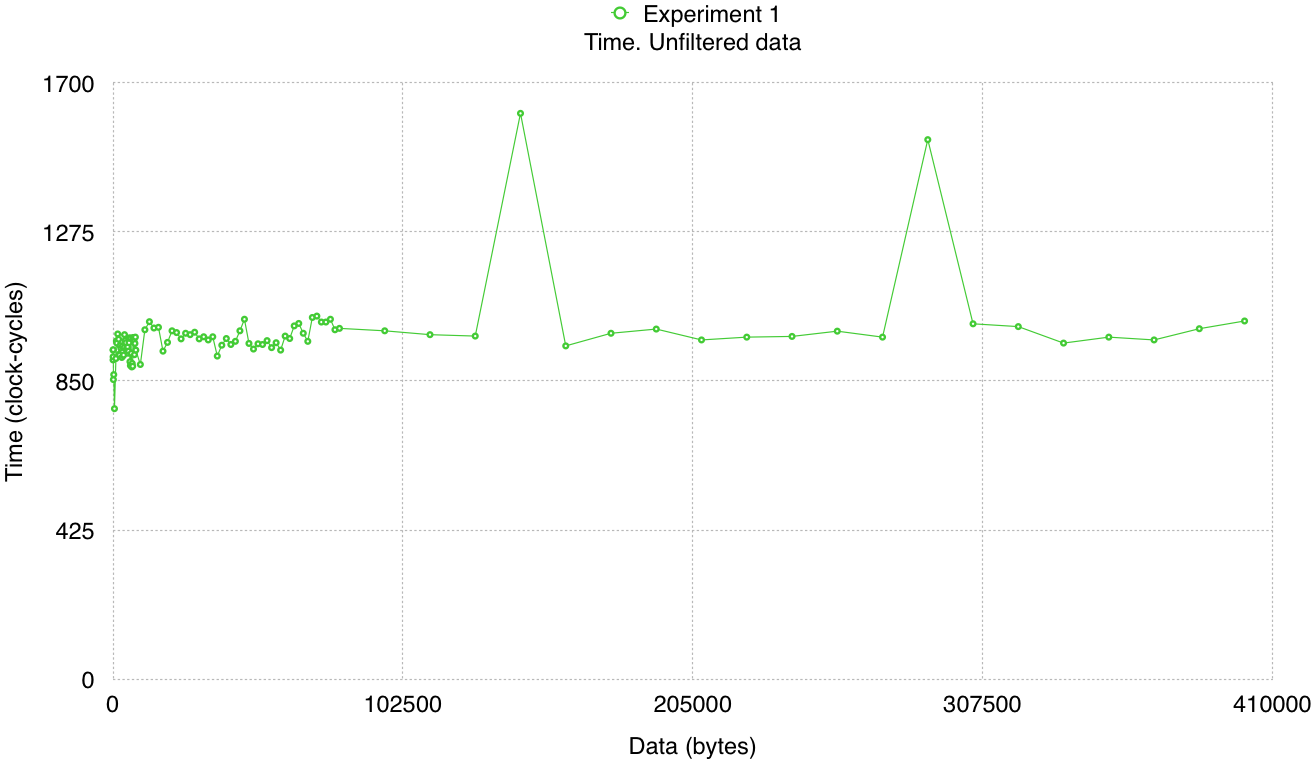
\includegraphics[width=145mm]{6/Cycle_experiment_dirty_ichec_small.png}
\caption{Xeon E5-2695 v2: data copying times, where $8 <= n <= 400064$ (unfiltered data, Experiment 1)}
\label{Cycle_experiment_dirty_ichec_small}
\end{figure}

A couple of ``big spikes" and a number of ``smaller spikes" may be seen on all graphs described in this section \ref{sec:cycle_results}, these abnormalities may be explained by the occurrence of interrupts and page faults that could not be filtered out, i.e. they were not only caused by the only unavoidable process that could be proven as such that generated minor page faults – opening files – and thus were caused by other processes run by the OS. On a smaller scale, where a small amount of data is shared between threads ($< 1000$ bytes), such behaviour may be explained by the fact that data is fetched from cache in pieces of information that are dividable by the size of a cache line. Also, one may argue that because it was not clear if hyper-threading is disabled on the Xeon E5-2695 v2, it may have had an impact as well. The experiments were run multiple times, but each time such abnormalities could not be isolated out.

In the end, the testing environment could not be configured to remove all overhead caused by the Operating System and all other processes that are executed when cycle-level experiments are run. Information on latency of cache and main memory was measured with lmbench, as described in the following section.

\subsection{Measuring Latency of Cache with lmbench}
\label{results_lmbench}

The lmbench tool reports that the Xeon 5130 machine has 0.5 ns timer accuracy and the Xeon E5-2695 v2 has 0.25 ns timer accuracy. Together with the chief technician of the faculty the author examined the source code of lmbench, which allowed to evaluate methods that are used in the benchmark. This evaluation revealed that it was not possible to configure the way the programme chooses its stride for ``jumping" between data samples. The stride value is important as it allows to configure the size of the buffer that is used in the benchmark; a correct value of this parameter will make sure that no levels of memory can be ``jumped over".

Figure \ref{lmbench_nuim} shows results of running \textit{lat\_mem\_rd} on the Xeon 5130. The x-axis represents the amount of data that is written into memory, the y-axis shows how many nano-seconds writing that data into memory takes. This plot shows how latency increases when the amount of data written into memory approaches the size of Level 2 cache, when data has to be written into main memory (more data is exchanged between threads that can fit into cache), the graph starts to flatten out.

\begin{figure}[!htb]
\centering
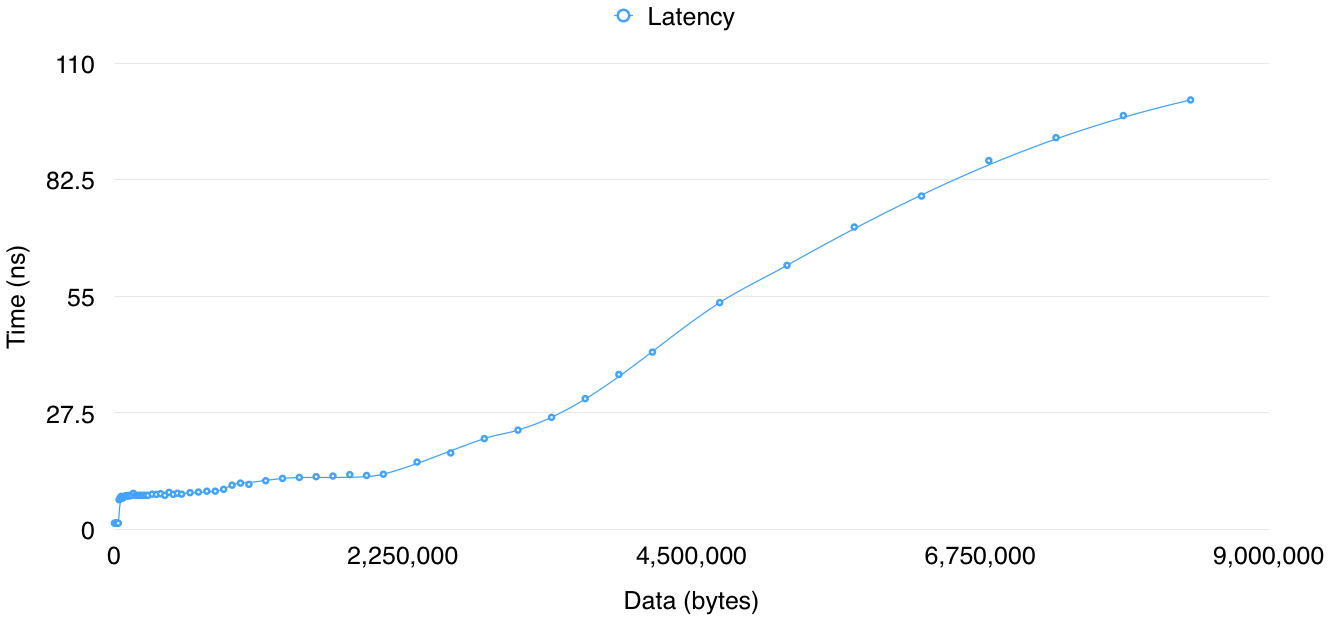
\includegraphics[width=145mm]{6/lmbench_nuim.png}
\caption{Xeon 5130: latency of cache, measured with lmbench}
\label{lmbench_nuim}
\end{figure}

Figure \ref{lmbench_ichec} shows results of running \textit{lat\_mem\_rd} on the Xeon E5-2695 v2. Similar to the figure \ref{lmbench_nuim}, the x-axis represents the amount of data that is written into memory, the y-axis shows how many nano-seconds writing that data into memory takes. Similar to figure \ref{lmbench_nuim}, one can see a ``jump" when the amount of data exchanged between threads approaches the size of Level 3 cache, then it gradually flattens out, as data is written into main memory at that stage. 

\begin{figure}[!htb]
\centering
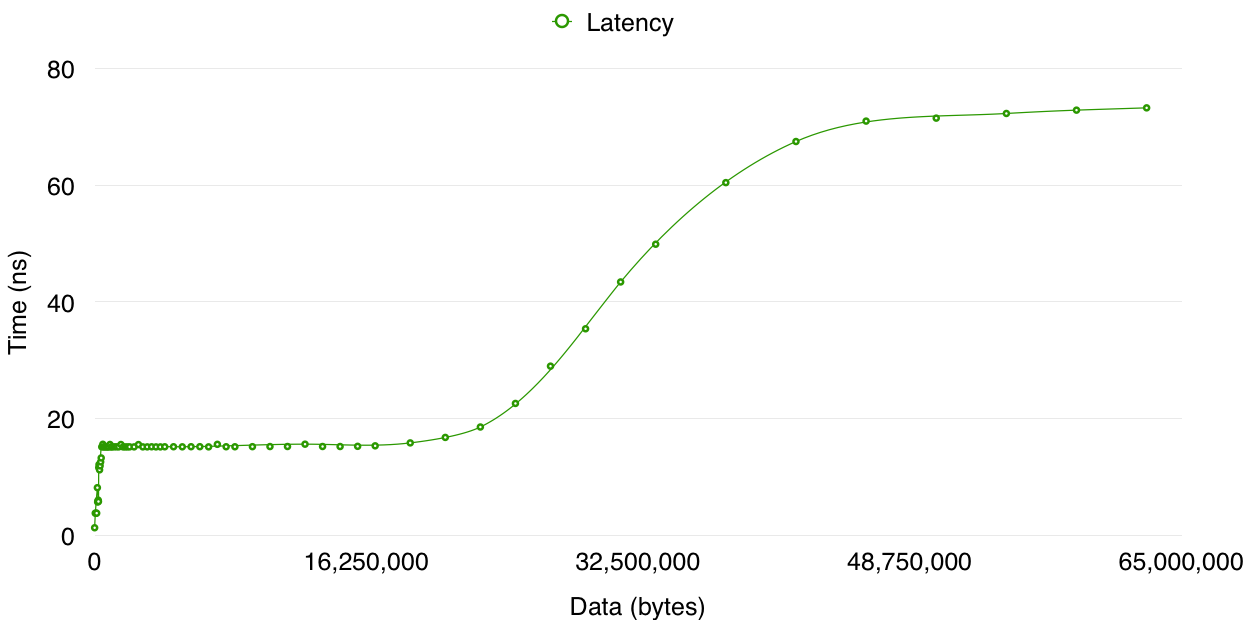
\includegraphics[width=145mm]{6/lmbench_ichec.png}
\caption{Xeon E5-2695 v2: latency of cache, measured with lmbench}
\label{lmbench_ichec}
\end{figure}

As was described in section \ref{conducting_cycle}, lmbench was difficult to operate. Mixed results were received. However, when the \textit{./cache} application was discovered, it became possible to verify assumptions made by running the \textit{lat\_mem\_rd} benchmark. Refer to table \ref{lmbenchTable} for results received from executing the \textit{./cache} programme. Close examination of the figures \ref{lmbench_nuim} and \ref{lmbench_ichec} and data presented in Appendix \ref{app:lmbench-results} shows that both benchmarks indicate the same values of latency of cache and memory. One may notice ``jumps" when the sizes of levels of cache are reached on the graphs.

\begin{table*}
\caption{Latency of cache and main memory as reported by lmbench}
\centering 
\begin{tabular}{lllll}
             & L1 cache & L2 cache & L3 cache & Main memory \\
Xeon 5130  & 1.5      & 7.0      & None     & 100.0         \\
Xeon E5-2695 v2 & 1.25     & 3.75     & 15.5     & 60.0       
\end{tabular}
\label{lmbenchTable}
\end{table*}

Results achieved by executing cycle-level experiments allowed to derive values of latency in two distinctly-different environments that are used in chapter \ref{discussionChapter} to discuss the model presented in chapter \ref{chapterModel}.

\section{Application-Level Experiments. Experiments 2 -- 4}
\label{results_app_experiments}

Figures \ref{App_experiment_1_throughput_dirty_nuim} and \ref{App_experiment_1_throughput_dirty_ichec} show unfiltered data measured through running three application-level experiments on the Xeon 5130 and the Xeon E5-2695 v2. In both cases, the x-axis represents the amount of data that is exchanged between threads, the y-axis shows the throughput ($n / t$, where $n$ indicated the amount of data exchanged between threads and $t$ represents the amount of time spent of exchanging the data).

\begin{figure}[!htb]
\centering
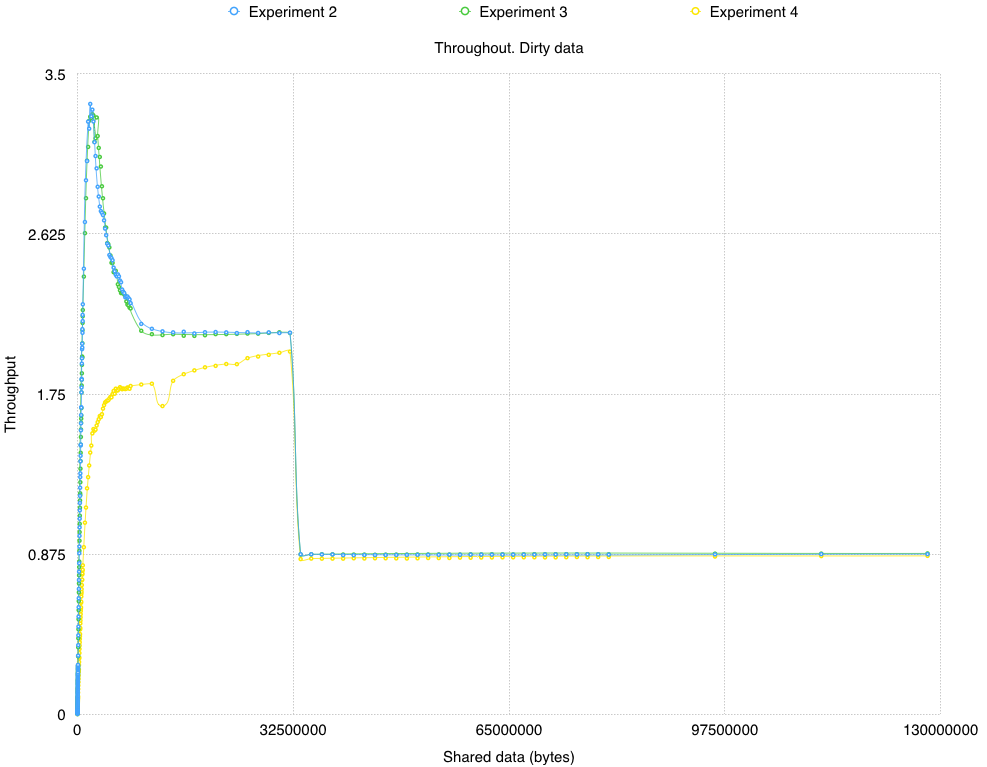
\includegraphics[width=145mm]{6/App_experiment_1_dirty_throughput_nuim.png}
\caption{Xeon 5130: throughput of copying data in inter-thread communication (Experiments 2-4)}
\label{App_experiment_1_throughput_dirty_nuim}
\end{figure}

\begin{figure}[!htb]
\centering
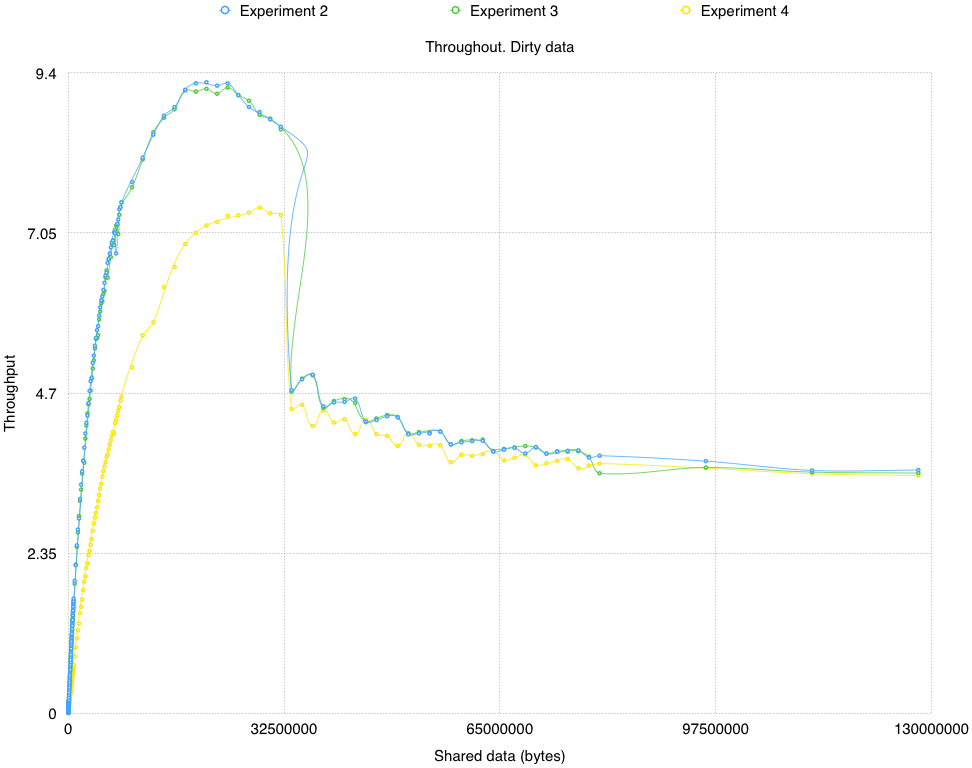
\includegraphics[width=145mm]{6/App_experiment_1_dirty_throughput_ichec.png}
\caption{Xeon E5-2695 v2: throughput of copying data in inter-thread communication (Experiments 2-4)}
\label{App_experiment_1_throughput_dirty_ichec}
\end{figure}

Both graphs exhibit decrease of throughput when the amount of shared between threads data exceeds 33600064 bytes (32.0435 MB). The fact that such behaviour was observed and on both systems with different architectures was not anticipated. The graph \ref{App_experiment_1_throughput_dirty_ichec} also shows ``waves" after reaching the 32.0435 MB mark. It is expected that all data larger than the size of Level 3 cache (30 MB) should be placed in the main memory, provided that it is smaller than the size of main memory. Therefore, no fluctuations could be expected.

As with results achieved by running the cycle-level experiments, detailed unfiltered results of first three runs of all iterations of the experiments with an indication of the numbers of interrupts and minor page faults that were recorded while running the experiments may be found in the following appendices:

\begin{itemize}
  \item Experiment 2 executed on the Xeon 5130: appendix \ref{app:app-level-results-2-nuim};
  \item Experiment 2 executed on the Xeon E5-2695 v2: appendix \ref{app:app-level-results-2-ichec};
  \item Experiment 3 executed on the Xeon 5130: appendix \ref{app:app-level-results-3-nuim};
  \item Experiment 3 executed on the Xeon E5-2695 v2: appendix \ref{app:app-level-results-3-ichec};
  \item Experiment 4 executed on the Xeon 5130: appendix \ref{app:app-level-results-4-nuim};
  \item Experiment 4 executed on the Xeon E5-2695 v2: appendix \ref{app:app-level-results-4-ichec}.
\end{itemize}

% \begin{figure}[!htb]
% \centering
% \includegraphics[width=145mm]{6/App_experiment_1_dirty_time_nuim.png}
% \caption{Results from the application-level experiment (time, unfiltered data). On the Xeon 5130. \hl{PLOT IN R}}
% \label{App_experiment_1_time_dirty_nuim}
% \end{figure}

% \begin{figure}[!htb]
% \centering
% \includegraphics[width=145mm]{6/App_experiment_1_dirty_time_ichec.png}
% \caption{Results from the application-level experiment (time, unfiltered data). On the Xeon E5-2695 v2. \hl{PLOT IN R}}
% \label{App_experiment_1_time_dirty_ichec}
% \end{figure}

Similar to the cycle-level experiments, running the application-level experiments within the experimental environment built for this project could not be configured in a way that would allow to receive accurate and fully-filtered data. Nevertheless, due to the nature of the application-level experiments that were run in the scope of this research, timing results that together with duration of the actual experiments also incorporate overhead caused by the operating system, may also be seen as satisfactory. More specifically, page faults, interrupts and other unwanted processes take considerably less time than the actual tests. Filtered data may be ignored as it was impossible to find a way to control the overhead imposed by the OS.

Finally, the overhead of the Operating System was measured for all three cases of inter-thread communication (described in Section \ref{taxonomy}). Such measurement was done by executing experiments with no data exchanged between two threads, i.e. only overhead of creating threads, creating a mutex, joining threads, and freeing memory was recorded. Each experiment was performed 1000 times and standard deviation (SD) was also calculated. Table \ref{overheadTable} gives a summary of the amount of overhead and its standard deviation (in nano-seconds) of performing the aforementioned operations. The standard deviation in all cases is not large: 1 -- 4\%.

\begin{table*}
\caption{Overhead of inter-thread communication}
\centering 
\begin{tabular}{llll}
             & Experiment 2 & Experiment 3 & Experiment 4 \\
Xeon 5130 (overhead) & 291408       & 297691       & 699229       \\
Xeon 5130 (SD) & 6320      & 5095       & 11694      \\
Xeon E5-2695 v2 (overhead) & 413963       & 415428       & 1073144 \\
Xeon E5-2695 v2 (SD) & 10130       & 12584       & 37449 
\end{tabular}
\label{overheadTable}
\end{table*}

\section{Measuring Duration of Interrupts and Minor Page Faults}
\label{resultsDurationIntPf}

Section \ref{modelsection} outlines the equations associated with the model. The duration of interrupts and minor page faults is measured because such data is needed to parametrise the model. Measured values are utilised to define $I_{ics}$ and $I_{pf\_min}$. Refer to appendix \ref{app:durationIntNuim} for the output of the programme \textit{test\_time\_int\_pf} for the Xeon 5130 (measured in nano-seconds). ``Num 1" should be ignored, it is used to avoid compiler optimisation. Appendix \ref{app:durationIntIchec} presents output of the application \textit{test\_time\_int\_pf} executed on the Xeon E5-2695 v2. As in the previous case, ``Num 1" should be ignored, it is used to avoid compiler optimisation. This test reported that an interrupt takes more than twice more time on this processor than on the Xeon 5130: 322826 ns (standard deviation: 17043 ns). Page faults are two times faster if compared to what is observed on the Xeon 5130: 21733 ns (standard deviation: 3162 ns). The results are presented in table \ref{intpfTable}.

\begin{table*}
\caption{Average duration of interrupts and minor page faults}
\centering 
\begin{tabular}{lll}
                            & Interrupt & Minor page fault \\
Xeon 5130 (duration)        & 153694       & 42666  \\
Xeon 5130 (SD)              & 175825      & 2471    \\
Xeon E5-2695 v2 (duration)  & 322826       & 21733 \\
Xeon E5-2695 v2 (SD)        & 17043     & 3162
\end{tabular}
\label{intpfTable}
\end{table*}

It may be observed that on average one interrupt takes 153694 ns (standard deviation: 175825 ns) and one minor page fault takes 42666 ns (standard deviation: 2471 ns). These figures represent unacceptable amounts of time in the case of cycle-level experiments.

% ---------------------------------------------------------------------------
%: ----------------------- end of thesis sub-document ------------------------
% ---------------------------------------------------------------------------